% Options for packages loaded elsewhere
\PassOptionsToPackage{unicode}{hyperref}
\PassOptionsToPackage{hyphens}{url}
%
\documentclass[
  x11names]{article}
\usepackage{amsmath,amssymb}
\usepackage{lmodern}
\usepackage{iftex}
\ifPDFTeX
  \usepackage[T1]{fontenc}
  \usepackage[utf8]{inputenc}
  \usepackage{textcomp} % provide euro and other symbols
\else % if luatex or xetex
  \usepackage{unicode-math}
  \defaultfontfeatures{Scale=MatchLowercase}
  \defaultfontfeatures[\rmfamily]{Ligatures=TeX,Scale=1}
\fi
% Use upquote if available, for straight quotes in verbatim environments
\IfFileExists{upquote.sty}{\usepackage{upquote}}{}
\IfFileExists{microtype.sty}{% use microtype if available
  \usepackage[]{microtype}
  \UseMicrotypeSet[protrusion]{basicmath} % disable protrusion for tt fonts
}{}
\makeatletter
\@ifundefined{KOMAClassName}{% if non-KOMA class
  \IfFileExists{parskip.sty}{%
    \usepackage{parskip}
  }{% else
    \setlength{\parindent}{0pt}
    \setlength{\parskip}{6pt plus 2pt minus 1pt}}
}{% if KOMA class
  \KOMAoptions{parskip=half}}
\makeatother
\usepackage{xcolor}
\usepackage[margin=1in]{geometry}
\usepackage{graphicx}
\makeatletter
\def\maxwidth{\ifdim\Gin@nat@width>\linewidth\linewidth\else\Gin@nat@width\fi}
\def\maxheight{\ifdim\Gin@nat@height>\textheight\textheight\else\Gin@nat@height\fi}
\makeatother
% Scale images if necessary, so that they will not overflow the page
% margins by default, and it is still possible to overwrite the defaults
% using explicit options in \includegraphics[width, height, ...]{}
\setkeys{Gin}{width=\maxwidth,height=\maxheight,keepaspectratio}
% Set default figure placement to htbp
\makeatletter
\def\fps@figure{htbp}
\makeatother
\setlength{\emergencystretch}{3em} % prevent overfull lines
\providecommand{\tightlist}{%
  \setlength{\itemsep}{0pt}\setlength{\parskip}{0pt}}
\setcounter{secnumdepth}{-\maxdimen} % remove section numbering
\usepackage{fontspec} \usepackage{titling} \pretitle{\begin{center} \vspace{-3cm}
\includegraphics[width=\linewidth]{images/Base_info/logo.png}\LARGE\\} \posttitle{\end{center}} \usepackage{float} \usepackage{fancyhdr} \usepackage{ragged2e} \usepackage{caption} \usepackage{colortbl} \captionsetup[figure]{labelformat=empty} \arrayrulecolor{white} \pagestyle{fancy} \fancyhead[L,C]{} \fancypagestyle{plain}{\pagestyle{fancy}} \PassOptionsToPackage{dvipsnames,svgnames*,x11names*}{xcolor} \definecolor{ceil}{rgb}{0.57, 0.63, 0.81} \usepackage[export]{adjustbox} \usepackage{wrapfig} \usepackage{graphicx} \usepackage{caption}
\usepackage{booktabs}
\usepackage{longtable}
\usepackage{array}
\usepackage{multirow}
\usepackage{wrapfig}
\usepackage{float}
\usepackage{colortbl}
\usepackage{pdflscape}
\usepackage{tabu}
\usepackage{threeparttable}
\usepackage{threeparttablex}
\usepackage[normalem]{ulem}
\usepackage{makecell}
\usepackage{xcolor}
\ifLuaTeX
  \usepackage{selnolig}  % disable illegal ligatures
\fi
\IfFileExists{bookmark.sty}{\usepackage{bookmark}}{\usepackage{hyperref}}
\IfFileExists{xurl.sty}{\usepackage{xurl}}{} % add URL line breaks if available
\urlstyle{same} % disable monospaced font for URLs
\hypersetup{
  hidelinks,
  pdfcreator={LaTeX via pandoc}}

\author{}
\date{\vspace{-2.5em}Fecha de creación: 03 April, 2023}

\begin{document}

\setmainfont{Arial}
\setsansfont{Arial}
\setmonofont{Arial}

\newcommand\invisiblesection[1]{%
  \refstepcounter{section}%
  \addcontentsline{toc}{section}{\protect\numberline{\thesection}#1}%
  \sectionmark{#1}}

\fancyhead[R]{\textbf{http://doi.org/10.31687/SaremLR.19.210}}

%
  \refstepcounter{section}%
  \addcontentsline{toc}{section}{\protect\numberline{\thesection}GENERALIDADES}%
  \sectionmark{GENERALIDADES}
\vspace{-0.4cm}


\includegraphics[width=1\linewidth]{images/Base_info/logo}

\vspace{1cm}

\begin{minipage}{0.7\textwidth}
\vspace{0.3cm}
\fontsize{20}{24}\selectfont\textit{Mazama americana}

\vspace{0.3cm}
\fontsize{30}{36}\selectfont Corzuela colorada
\end{minipage}
\hspace{0.05\textwidth}
\begin{minipage}{0.25\textwidth}

\includegraphics[width=\textwidth]{images/vu.png}
\end{minipage}

\normalsize

\begin{figure}[H]

{\centering 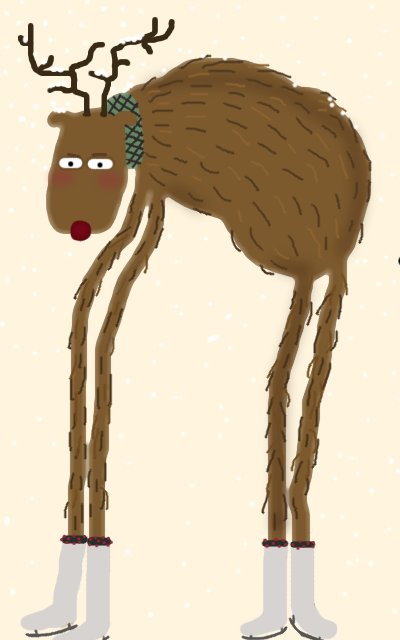
\includegraphics[width=0.35\linewidth]{photos/Blastocerus dichotomus} 

}

\caption{Fotos por Salvador Dali}\label{fig:image}
\end{figure}

\begin{center}\rule{0.5\linewidth}{0.5pt}\end{center}

\justifying

\textbf{Citar como:} Varela, Diego; de Bustos, Soledad; Di Bitetti,
Mario S.; Cirignoli, Sebastián. (2019). \emph{Mazama americana}. En:
SAyDS--SAREM (eds.) Categorización 2019 de los mamíferos de Argentina
según su riesgo de extinción. Lista Roja de los mamíferos de Argentina.
\url{http://doi.org/10.31687/SaremLR.19.210}

\begin{center}\rule{0.5\linewidth}{0.5pt}\end{center}

\newpage

%
  \refstepcounter{section}%
  \addcontentsline{toc}{section}{\protect\numberline{\thesection}ÁREA DE DISTRIBUCIÓN ACTUAL}%
  \sectionmark{ÁREA DE DISTRIBUCIÓN ACTUAL}
\begin{table}[H]
\centering
\begin{tabular}[t]{>{\raggedright\arraybackslash}m{16cm}>{}m{16cm}}
\toprule
\cellcolor{ceil}{\textcolor{white}{\textbf{\rule{0pt}{14pt}ÁREA DE DISTRIBUCIÓN ACTUAL}}}\\
\bottomrule
\end{tabular}
\end{table}

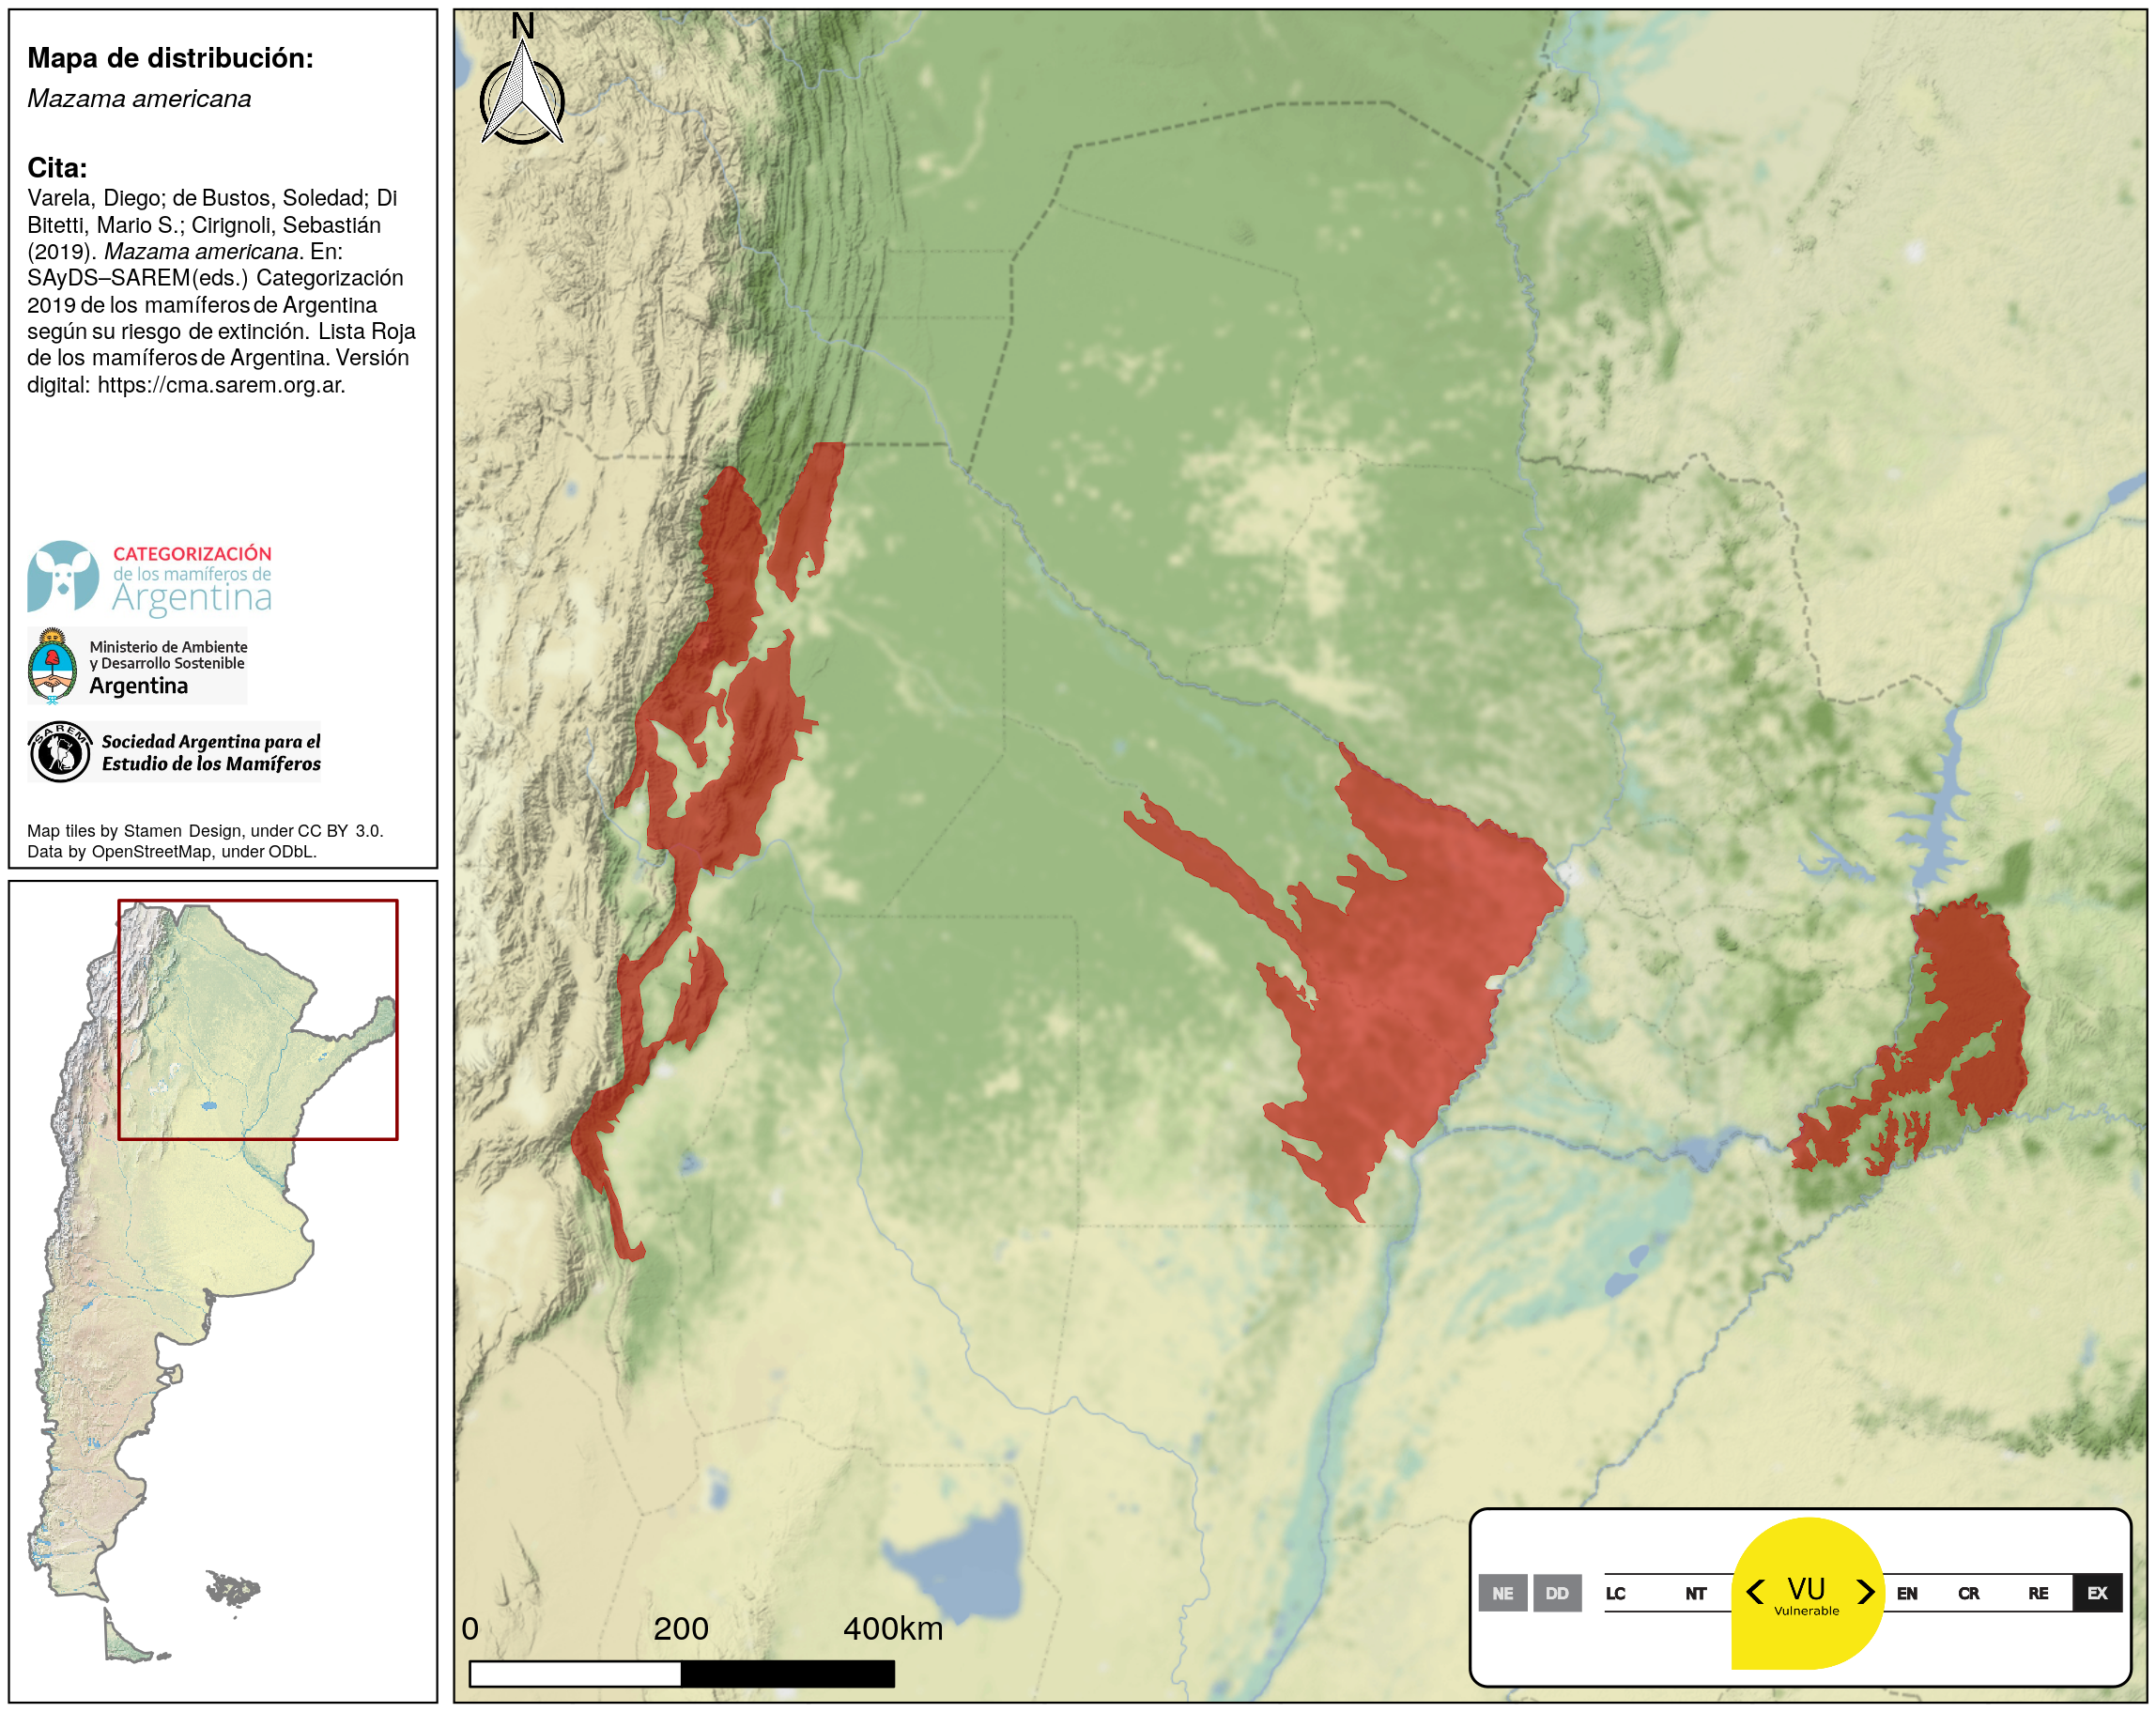
\includegraphics[width=1\linewidth]{maps/Cetartiodactyla/Mazama_americana}

%
  \refstepcounter{section}%
  \addcontentsline{toc}{section}{\protect\numberline{\thesection}CATEGORÍAS DE CONSERVACIÓN}%
  \sectionmark{CATEGORÍAS DE CONSERVACIÓN}
\begin{table}[H]
\centering
\begin{tabular}[t]{>{\raggedright\arraybackslash}m{16cm}>{}m{16cm}}
\toprule
\cellcolor{ceil}{\textcolor{white}{\textbf{\rule{0pt}{14pt}CATEGORÍAS DE CONSERVACIÓN}}}\\
\bottomrule
\end{tabular}
\end{table}

\vspace{-0.4cm}

\textbf{Categoría Nacional de Conservación 2019}

VU (Vulnerable)

\textbf{Criterios y subcriterios}

A2cde

\textbf{Justificación de la categorización}

Mazama americana es una especie cuyo hábitat depende de una buena
cobertura de bosques húmedos y es sensible a la cacería. Su estatus
taxonómico actual es incierto y se cree que la forma Mazama americana
engloba varias especies crípticas. La especie está presente en las
ecorregiones de~ Selva Paranaense, Chaco Húmedo y Yungas. En las últimas
3 generaciones se observó proceso de pérdida, degradación y
fragmentación del hábitat de la corzuela colorada, que lleva también al
incremento de otras amenazas como la cacería, el hostigamiento y
depredación por perros, y el atropellamiento en rutas. En Misiones la
especie es más frecuente en bosques continuos con baja presión de
cacería y en áreas protegidas, pero desaparece en áreas fragmentadas
afectadas por la cacería y la presencia de perros (Di Bitetti et
al.~2008) y podría haber desaparecido en la mayoría de los fragmentos de
bosque del sur de la provincia, donde el guazuncho (Mazama gouazoubira)
es más frecuente. En Yungas ha desaparecido de las Selvas Pedemontanas,
donde el guazuncho sigue siendo muy abundante (Albanesi et al.~en
prensa;~Di Bitetti et al.~2013), probablemente a causa de los desmontes
y la elevada cacería.~ Persiste en las selvas y bosques montanos, aunque
es afectada por la cacería y la competencia con el ganado y, al menos en
las porciones más bajas de las selvas montanas es mucho menos frecuente
que el guazuncho (Di Bitetti et al.~2013). La situación en el Chaco
Húmedo es incierta, su hábitat está sujeto a fuertes desmontes para el
desarrollo de la agricultura y la ganadería, pero la especie persiste en
algunas áreas protegidas y formaciones de bosques húmedos asociados a
los riachos. En función de estas amenazas, estimamos y sospechamos que
las poblaciones de la especie se han reducido en más de un 30\% en todo
su rango de distribución~ en las últimas 3 generaciones (criterio A2),
en función de la reducción en: 1) la extensión de la presencia (EOO), el
área de ocupación (AOO) y la calidad del hábitat (subcriterio c) , 2)
niveles de explotación~ debido a la caza furtiva y caza de subsistencia,
depredación por perros domésticos y en menor medida, atropellamientos
(subcriterio d) y competencia con el ganado, particularmente en Yungas
(subcriterio e). Por lo tanto, consideramos que la especie se encuentra
actualmente en la categoría de Vulnerable (VU). El efecto rescate de
poblaciones de países vecinos tiene una probabilidad alta en el norte de
las Yungas, pero con probabilidad baja en las otras dos subpoblaciones.
El cambio de categoría con respecto a 2012 es considerado genuino, como
consecuencia al aumento en sus amenazas.

\textbf{Evaluación de subpoblaciones locales}

\begin{tabu} to \linewidth {>{\raggedright}X>{\raggedright}X>{\raggedright}X}
\toprule
\textbf{Subpoblación} & \textbf{Categoría} & \textbf{Criterios y subcriterios}\\
\arrayrulecolor{white}
\midrule
\cellcolor{gray!6}{Selva Paranaense} & \cellcolor{gray!6}{VU (Vulnerable)} & \cellcolor{gray!6}{A2cde}\\
\bottomrule
\end{tabu}

\textbf{Justificación}

La especie es frecuente en bosques bien conservados y con baja presión
de cacería (Di Bitetti et al.~2008; Paviolo et al.~2009), como por
ejemplo, el Parque Nacional Iguazú. Utiliza plantaciones forestales de
pinos en áreas con bajos niveles de cacería y próximas a grandes bloques
de bosques nativos (Iezzi et al.~2018). Sin embargo, la ocupación y la
abundancia relativa es baja en bosques fragmentados, degradados y con
alta presión de caza furtiva (Di Bitetti et al.~2008). Estimamos que
hubo una reducción en el tamaño poblacional en el pasado (criterio A2)
mayor al 30\%, producto de la reducción en el EOO y AOO (subcriterio c),
una alta mortalidad por cacería ilegal (subcriterio d) y posible
competencia con M. gouazoubira (en bosques degradados y fragmentados) y
hostigamiento por perros (Subcriterio e).\vspace{0.5cm}

\begin{tabu} to \linewidth {>{\raggedright}X>{\raggedright}X>{\raggedright}X}
\toprule
\textbf{Subpoblación} & \textbf{Categoría} & \textbf{Criterios y subcriterios}\\
\arrayrulecolor{white}
\midrule
\cellcolor{gray!6}{Yungas} & \cellcolor{gray!6}{NT (Casi Amenazada)} & \cellcolor{gray!6}{A2cde}\\
\bottomrule
\end{tabu}

\textbf{Justificación}

Esta subpoblación se encuentra aislada del resto del área de
distribución argentina. En esta ecorregión se la considera Casi
Amenazada (NT) debido a la reducción de la población (Criterio A2) que
se infiere es ligeramente superior al 20\% en las últimas 3 generaciones
debido a la pérdida y degradación de su hábitat (subcriterio c),
principalmente en la Selva Pedemontana; también la fuerte presión de
caza furtiva (subcriterio d) y la competencia con el ganado vacuno
(subcriterio e). El hecho de que la especie habite mayormente áreas de
relieve fuertemente quebrado y de difícil acceso humano, la resguarda de
ciertas amenazas.\vspace{0.5cm}

\begin{tabu} to \linewidth {>{\raggedright}X>{\raggedright}X>{\raggedright}X}
\toprule
\textbf{Subpoblación} & \textbf{Categoría} & \textbf{Criterios y subcriterios}\\
\arrayrulecolor{white}
\midrule
\cellcolor{gray!6}{Chaco Húmedo} & \cellcolor{gray!6}{DD (Datos Insuficientes)} & \cellcolor{gray!6}{Se conoce muy poco de la distribución y abundancia de la especie en la región del Chaco Húmedo debido a la falta de relevamientos específicos, aunque sospechamos que se encuentra amenazada a causa de la pérdida y fragmentación del hábitat y la cacería. Tenemos registros de su presencia solo en algunas áreas naturales protegidas (Parque Nacional Pilcomayo, Parque Provincial Pampa del Indio, Reserva Privada Guaycolec).}\\
\bottomrule
\end{tabu}

\textbf{Justificación}

NA

NA

Se conoce muy poco de la distribución y abundancia de la especie en la
región del Chaco Húmedo debido a la falta de relevamientos específicos,
aunque sospechamos que se encuentra amenazada a causa de la pérdida y
fragmentación del hábitat y la cacería. Tenemos registros de su
presencia solo en algunas áreas naturales protegidas (Parque Nacional
Pilcomayo, Parque Provincial Pampa del Indio, Reserva Privada
Guaycolec).

\textbf{Categoría Res. SAyDS 1030/04}

NA (No Amenazada)

\textbf{Categorías nacionales de conservación previas (SAREM)}

\arrayrulecolor{white}

%
  \refstepcounter{section}%
  \addcontentsline{toc}{section}{\protect\numberline{\thesection}TAXONOMÍA Y NOMENCLATURA}%
  \sectionmark{TAXONOMÍA Y NOMENCLATURA}
\begin{table}[H]
\centering
\begin{tabular}[t]{>{\raggedright\arraybackslash}m{16cm}>{}m{16cm}}
\toprule
\cellcolor{ceil}{\textcolor{white}{\textbf{\rule{0pt}{14pt}TAXONOMÍA Y NOMENCLATURA}}}\\
\bottomrule
\end{tabular}
\end{table}

%
  \refstepcounter{section}%
  \addcontentsline{toc}{section}{\protect\numberline{\thesection}INFORMACIÓN RELEVANTE PARA LA EVALUACIÓN}%
  \sectionmark{INFORMACIÓN RELEVANTE PARA LA EVALUACIÓN}
\begin{table}[H]
\centering
\begin{tabular}[t]{>{\raggedright\arraybackslash}m{16cm}>{}m{16cm}}
\toprule
\cellcolor{ceil}{\textcolor{white}{\textbf{\rule{0pt}{14pt}INFORMACIÓN RELEVANTE PARA LA EVALUACIÓN}}}\\
\bottomrule
\end{tabular}
\end{table}

%
  \refstepcounter{section}%
  \addcontentsline{toc}{section}{\protect\numberline{\thesection}RANGO GEOGRÁFICO, OCURRENCIA Y ABUNDANCIA Y NOMENCLATURA}%
  \sectionmark{RANGO GEOGRÁFICO, OCURRENCIA Y ABUNDANCIA Y NOMENCLATURA}
\begin{table}[H]
\centering
\begin{tabular}[t]{>{\raggedright\arraybackslash}m{16cm}>{}m{16cm}}
\toprule
\cellcolor{ceil}{\textcolor{white}{\textbf{\rule{0pt}{14pt}RANGO GEOGRÁFICO, OCURRENCIA Y ABUNDANCIA Y NOMENCLATURA}}}\\
\bottomrule
\end{tabular}
\end{table}

%
  \refstepcounter{section}%
  \addcontentsline{toc}{section}{\protect\numberline{\thesection}DATOS MORFOMÉTRICOS}%
  \sectionmark{DATOS MORFOMÉTRICOS}
\begin{table}[H]
\centering
\begin{tabular}[t]{>{\raggedright\arraybackslash}m{16cm}>{}m{16cm}}
\toprule
\cellcolor{ceil}{\textcolor{white}{\textbf{\rule{0pt}{14pt}DATOS MORFOMÉTRICOS}}}\\
\bottomrule
\end{tabular}
\end{table}

%
  \refstepcounter{section}%
  \addcontentsline{toc}{section}{\protect\numberline{\thesection}RASGOS ETO-ECOLÓGICOS}%
  \sectionmark{RASGOS ETO-ECOLÓGICOS}
\begin{table}[H]
\centering
\begin{tabular}[t]{>{\raggedright\arraybackslash}m{16cm}>{}m{16cm}}
\toprule
\cellcolor{ceil}{\textcolor{white}{\textbf{\rule{0pt}{14pt}RASGOS ETO-ECOLÓGICOS}}}\\
\bottomrule
\end{tabular}
\end{table}

%
  \refstepcounter{section}%
  \addcontentsline{toc}{section}{\protect\numberline{\thesection}CONSERVACIÓN E INVESTIGACIÓN}%
  \sectionmark{CONSERVACIÓN E INVESTIGACIÓN}
\begin{table}[H]
\centering
\begin{tabular}[t]{>{\raggedright\arraybackslash}m{16cm}>{}m{16cm}}
\toprule
\cellcolor{ceil}{\textcolor{white}{\textbf{\rule{0pt}{14pt}CONSERVACIÓN E INVESTIGACIÓN}}}\\
\bottomrule
\end{tabular}
\end{table}

%
  \refstepcounter{section}%
  \addcontentsline{toc}{section}{\protect\numberline{\thesection}BIBLIOGRAFÍA}%
  \sectionmark{BIBLIOGRAFÍA}
\begin{table}[H]
\centering
\begin{tabular}[t]{>{\raggedright\arraybackslash}m{16cm}>{}m{16cm}}
\toprule
\cellcolor{ceil}{\textcolor{white}{\textbf{\rule{0pt}{14pt}BIBLIOGRAFÍA}}}\\
\bottomrule
\end{tabular}
\end{table}

\newpage

%
  \refstepcounter{section}%
  \addcontentsline{toc}{section}{\protect\numberline{\thesection}AUTORES}%
  \sectionmark{AUTORES}
\begin{table}[H]
\centering
\begin{tabular}[t]{>{\raggedright\arraybackslash}m{16cm}>{}m{16cm}}
\toprule
\cellcolor{ceil}{\textcolor{white}{\textbf{\rule{0pt}{14pt}AUTORES}}}\\
\bottomrule
\end{tabular}
\end{table}

\textbf{AUTORES}

\begin{tabu} to \linewidth {>{}l>{\raggedright\arraybackslash}p{2cm}>{\raggedright}X}
\toprule
\textbf{\cellcolor{gray!6}{Cirignoli, Sebastián}} & \cellcolor{gray!6}{} & \cellcolor{gray!6}{Centro de Investigaciones del Bosque Atlántico (CeIBA), Puerto Iguazú, Misiones, Argentina}\\
\textbf{de Bustos, Soledad} &  & Secretaría de Ambiente y Desarrollo Sustentable de la Provincia de Salta y Fundación Biodiversidad, Salta, Salta, Argentina\\
\textbf{\cellcolor{gray!6}{Di Bitetti, Mario S.}} & \cellcolor{gray!6}{} & \cellcolor{gray!6}{Instituto de Biología Subtropical (IBS), CONICET-Universidad Nacional de Misiones, Facultad de Ciencias Forestales (FACFOR-UNaM) y Centro de Investigaciones del Bosque Atlántico (CeIBA), Puerto Iguazú, Misiones, Argentina}\\
\textbf{Varela, Diego} &  & Instituto de Biología Subtropical (IBS), CONICET-Universidad Nacional de Misiones y Centro de Investigaciones del Bosque Atlántico (CeIBA), Puerto Iguazú, Misiones, Argentina\\
\bottomrule
\end{tabu}

\textbf{COLABORADORES}

\begin{tabu} to \linewidth {>{}l>{\raggedright\arraybackslash}p{2cm}>{\raggedright}X}
\toprule
\textbf{\cellcolor{gray!6}{Albanesi, Sebastián}} & \cellcolor{gray!6}{} & \cellcolor{gray!6}{Instituto de Biodiversidad Neotropical, Universidad Nacional de Tucumán - CONICET, Yerba Buena, Tucumán, Argentina}\\
\textbf{Camino, Micaela} &  & Laboratorio de Biología de la Conservación, Centro de Ecología Aplicada del Litoral (CECOAL) - CONICET, Corrientes, Argentina\\
\textbf{\cellcolor{gray!6}{de la Colina, Alicia}} & \cellcolor{gray!6}{} & \cellcolor{gray!6}{Fundación Temaikén, Escobar, Buenos Aires, Argentina}\\
\textbf{Giraudo, Alejandro R.} &  & Laboratorio de Biodiversidad y Conservación de Tetrápodos, Instituto Nacional de Limnología (INALI), Univerisidad Nacional del Litoral - CONICET, Santa Fe, Santa Fe, Argentina\\
\textbf{\cellcolor{gray!6}{Nicéforo, Luna}} & \cellcolor{gray!6}{} & \cellcolor{gray!6}{Guardaparques provinciales, Secretaría de Ambiente y Desarrollo Sustentable de la Provincia de Salta, Salta, Argentina}\\
\addlinespace
\textbf{Quiroga, Verónica A.} &  & Instituto de Diversidad y Ecología Animal (IDEA - CONICET), Centro de Zoología Aplicada, Universidad Nacional de Córdoba - Centro de Investigaciones del Bosque Atlántico (CeIBA), Córdoba, Argentina\\
\textbf{\cellcolor{gray!6}{Teta, Pablo}} & \cellcolor{gray!6}{} & \cellcolor{gray!6}{División Mastozoología, Museo Argentino de Ciencias Naturales Bernardino Rivadavia (MACN-CONICET), CABA, Argentina}\\
\textbf{Torresín, Jerónimo} &  & Fundación Temaikén, Posadas, Misiones, Argentina\\
\textbf{\cellcolor{gray!6}{Trucco, Carlos}} & \cellcolor{gray!6}{} & \cellcolor{gray!6}{Parque Nacional Río Pilcomayo, Administración de Parques Nacionales, Formosa, Argentina}\\
\bottomrule
\end{tabu}

\end{document}
